\newgeometry{left=1.50cm, right=1.25cm}
\begin{figure}
  \section{MAPA DA UFSCAR}
  \begin{vwcol}[widths={0.6,0.4}, rule=0pt]
    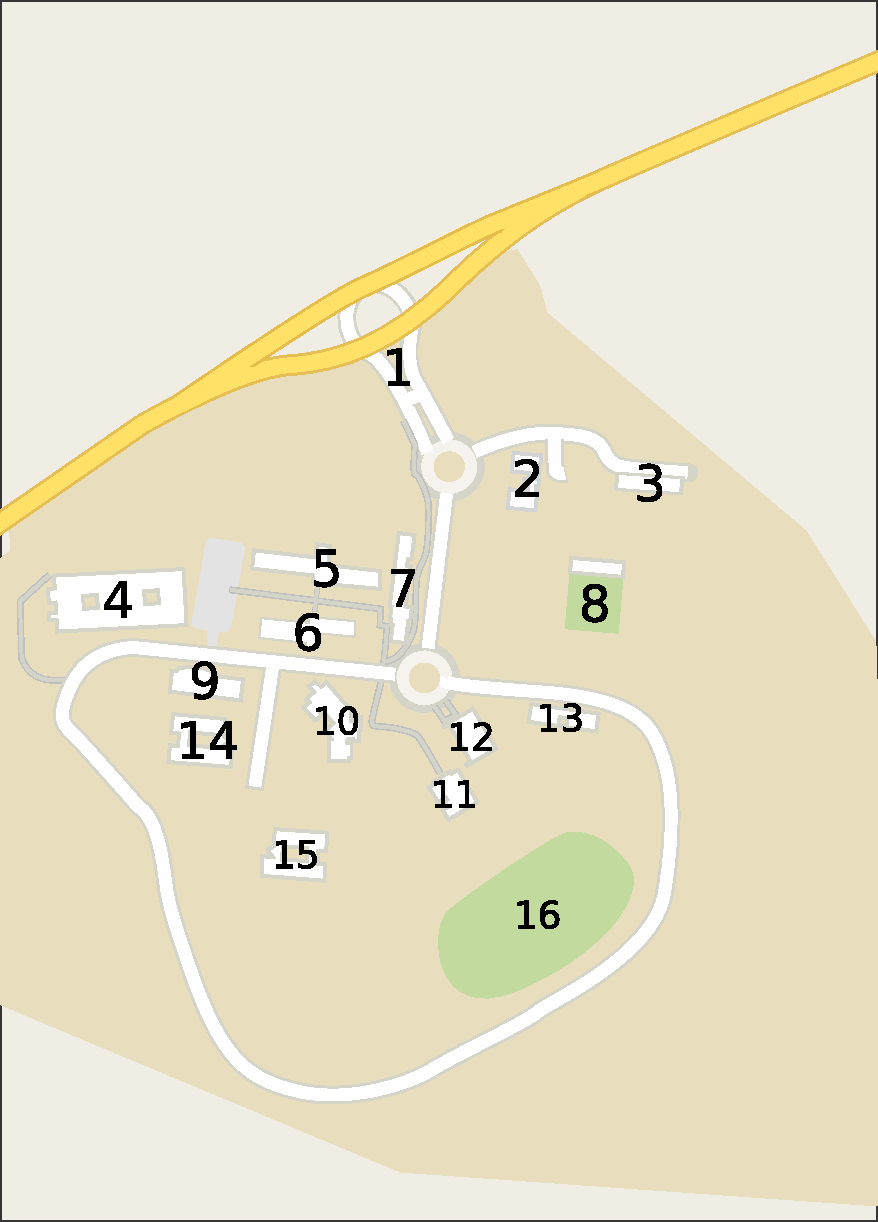
\includegraphics[width=0.6\textwidth]{./imagem/image.pdf}
    \vfill
    \begin{enumerate}
      \item Portaria
      \item Administração
      \item Almoxarifado
      \item ATLab (Prédio Roxo)
      \item Laboratórios
      \item AT (Aulas Teóricas)
      \item DiGRA
      \item Quadra
      \item AT-2 (Prédio Vermelho)
      \item Biblioteca
      \item Área de Vivência
      \item Restaurante Universitário
      \item Ambulatório
      \item CCGT (Prédio Verde)
      \item CCTS (Prédio Amarelo)
      \item Pista de corrida/Campo de futebol
    \end{enumerate}
  \end{vwcol}

\end{figure}

\restoregeometry
